\documentclass[9pt, aspectratio=169]{beamer}
%\documentclass[9pt, aspectratio=169, handout]{beamer}

\usetheme{metropolis}
\setbeamertemplate{itemize items}{\faAngleRight}

\metroset{titleformat=smallcaps,block=fill,numbering=counter,progressbar=frametitle,sectionpage=none}
\setbeamersize{text margin left=5mm,text margin right=5mm} 
% \input{embed_video}
\usepackage{fontspec}
\usepackage[scale=1]{ccicons}
\usepackage{metalogo}
\usepackage{xcolor,colortbl}
\usepackage{multicol,multirow,booktabs}
\usepackage{appendixnumberbeamer}
\usepackage{graphicx}
\usepackage{svg}
\usepackage{mismath}
\usepackage{bm}
\usepackage{fontawesome5}
\usepackage{csquotes}
%\usepackage[backend=biber, natbib, sorting=nyt, doi=true, url=false, url=false, isbn=false, maxbibnames=10]{biblatex}
%\addbibresource{../../utils/refs.bib}

\usepackage[spanish, es-nodecimaldot]{babel}
\deftranslation[to=spanish]{Definition}{Definición}
\deftranslation[to=spanish]{Theorem}{Teorema}
\deftranslation[to=spanish]{Example}{Ejemplo}

\usepackage{mathtools, mathrsfs}
\usefonttheme{professionalfonts}
\usepackage{textcomp, wasysym}

\setsansfont[BoldFont={Iwona Bold}, Numbers={Lining, Proportional}]{Iwona Light}
% \setmathsfont(Digits)[Numbers={Lining, Proportional}]{Fira Sans Light}
\setmonofont[Scale=MatchLowercase]{DejaVu Sans Mono}

\setbeamercolor{alerted text}{fg=red,bg=black!2}
\setbeamercolor{progress bar}{fg=red,bg=red!2}
\setbeamertemplate{itemize item}{\faCaretRight}
\setbeamertemplate{itemize subitem}{ \faAngleRight}
\setbeamertemplate{blocks}[shadow=false]
\setbeamercolor{block title}{bg=black!30,fg=red}
\setbeamercolor{block body}{bg=black!20,fg=black}
\setbeamertemplate{theorem begin}
{%
\begin{\inserttheoremblockenv}
{%
\inserttheoremheadfont
%{Teorema:}
\inserttheoremname
\ifx\inserttheoremaddition\@empty\else\ : \inserttheoremaddition\fi%
\inserttheorempunctuation
}%
}
\setbeamertemplate{theorem end}{\end{\inserttheoremblockenv}}
\makeatother


 
\usepackage{gensymb,amssymb}
\usepackage{siunitx}
\DeclareSIUnit{\nada}{\relax}
\usepackage{upquote}
\usepackage{cancel}
\usepackage{algpseudocode}
\algrenewcommand\algorithmicrequire{\textbf{Requiere}}
\algrenewcommand\algorithmicensure{\textbf{Devuelve}}
\setbeamertemplate{blocks}[shadow=false]

\newcommand{\cx}{\column{0.5\textwidth}}
\newcommand{\cw}[1]{\column{#1\textwidth}}

\author{Manuel Carlevaro}
\date{}
\institute{
  \vspace{6em}
  \centering
  {\small
  Universidad de Navarra \enspace • \enspace 2024 
} }

%% Operadores
\DeclareMathOperator{\sen}{sen}
\DeclareMathOperator{\senc}{senc}
\DeclareMathOperator{\sign}{sign}
\newcommand{\T}[1]{\underline{\bm{#1}}}
\DeclareMathOperator{\Tr}{Tr}
\DeclareMathOperator{\rg}{rg}
\DeclareMathOperator{\cond}{cond}

\usepackage{hyperref}
\hypersetup{
    colorlinks,
    citecolor=blue,
    filecolor=black,
    linkcolor=blue,
    urlcolor=blue
}
\urlstyle{same}


\usepackage{tikz}
\usetikzlibrary{shapes,shadows,arrows,positioning,matrix,chains,backgrounds,fit}

\tikzset{
    %Define standard arrow tip
    >=stealth',
    %Define style for boxes
    obj/.style={
           rectangle,
           rounded corners,
           draw, very thick,
           text width=10em, fill=green!20,
           minimum height=2em,
           text centered, drop shadow},
    proc/.style={
	    rectangle, rounded corners,
	    draw,fill=red!50,very thick,
	    text width=8em,minimum height=2em,
	    text centered, drop shadow},
    % Define arrow style
    pil/.style={
           ->,
           thick,
           shorten <=2pt,
           shorten >=2pt,}
}

%\setbeamertemplate{bibliography item}{%
  %\ifboolexpr{ test {\ifentrytype{book}} or test {\ifentrytype{mvbook}}
    %or test {\ifentrytype{collection}} or test {\ifentrytype{mvcollection}}
    %or test {\ifentrytype{reference}} or test {\ifentrytype{mvreference}} }
    %{\setbeamertemplate{bibliography item}{\faBook}}
    %{\ifentrytype{online}
            %{\setbeamertemplate{bibliography item}{\faGlobe}}
   %{\setbeamertemplate{bibliography item}{\faFileText}}}%
  %\usebeamertemplate{bibliography item}}

%\defbibenvironment{bibliography}
  %{\list{}
     %{\settowidth{\labelwidth}{\usebeamertemplate{bibliography item}}%
      %\setlength{\leftmargin}{\labelwidth}%
      %\setlength{\labelsep}{\biblabelsep}%
      %\addtolength{\leftmargin}{\labelsep}%
      %\setlength{\itemsep}{\bibitemsep}%
      %\setlength{\parsep}{\bibparsep}}}
  %{\endlist}
  %{\item}
%\newcommand{\bcite}[1]{\citeauthor{#1}, \citetitle{#1} (\citeyear{#1})}


\title{Introducción a la física}
\subtitle{Dinámica}


\begin{document}
\maketitle
\begin{frame}
  \frametitle{Objetivos}
\Large

\begin{itemize}
 \item Recordar el concepto de fuerza.
 \item Repasar las tres leyes de Newton.
 \item Reforzar las técnicas de resolución de problemas de movimiento causado por fuerzas.
\end{itemize}
\end{frame}

\begin{frame}{Fuerza}
\begin{definition}[Fuerza]
    \textbf{Fuerza} es una \textbf{interacción} entre dos cuerpos o entre un cuerpo y su ambiente.
\end{definition}
\pause

\begin{columns} 
\cw{0.8}
\begin{itemize}
    \item Las fuerzas son magnitudes \textbf{vectoriales}.
    \item La unidad de fuerza en el S.I. es el Newton (N).
    \item Tipos de fuerza:
        \begin{itemize}
            \item De contacto: normal, fricción, tensión.
            \item A distancia: gravedad (peso), magnética, eléctrica, etc.
        \end{itemize}
    \item La magnitud de una fuerza se puede medir con una balanza de resorte (dinamómetro).
\end{itemize}
\begin{center}
    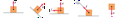
\includegraphics[width=0.9\textwidth]{figs/fig-01.pdf}
\end{center}
\cw{0.2}
\begin{center}
    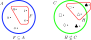
\includegraphics[height=0.4\textheight]{figs/fig-02.png}
    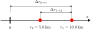
\includegraphics[width=0.8\textwidth]{figs/fig-03.png}
\end{center}
\end{columns}
\end{frame}

\begin{frame}{Principio de superposición}
\begin{center}
    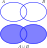
\includegraphics[width=0.5\textwidth]{figs/fig-04.pdf}
\end{center}
\begin{definition}[Principio de superposición]
El efecto de cualquier cantidad de fuerzas aplicadas a un punto  de un cuerpo es el mismo de una sola fuerza igual a la \textbf{suma vectorial} de las fuerzas.
\end{definition}
\pause

\begin{itemize}
    \item Es más simple expresar las fuerzas en componentes para hacer la suma vectorial y obtener $\vec{R}$ (fuerza \textbf{resultante} o \textbf{neta}).
    \item Si las fuerzas no están aplicadas sobre el mismo punto, el efecto de \textbf{traslación} es equivalente a aplicar la resultante sobre el centro de masa. \alert{Atención: el efecto de rotación no es equivalente}.
    \item El \textbf{diagrama de cuerpo libre} simplifica el cálculo de la resultante.
\end{itemize}
\end{frame}

\begin{frame}{Leyes de Newton}
\begin{block}{Primera ley de Newton}
Un cuerpo sobre el que no actúa una fuerza neta se mueve con velocidad constante (que puede ser cero) y aceleración cero.
\end{block}
\pause
\medskip

\begin{columns} 
\cx 
\textbf{Ejemplo.} Una cinta transportadora lleva una caja a \qty{0.2}{m/s} en una línea de montaje de una fábrica. ¿Es posible saber la fuerza resultante sobre la caja? ¿Qué fuerzas actúan sobre la caja? Al terminar la cinta la caja desliza sobre una mesa contigua y se detiene. ¿Es la fuerza neta igual a cero en este proceso?
\pause

\cx 
Cuando un cuerpo está en reposo o se mueve con velocidad constante (en línea recta con rapidez constante), decimos que esta en \textbf{equilibrio}. Para esto no deben actuar fuerzas, o deben actuar varias fuerzas para que la resultante sea cero:
\[ \sum_i \vect{F}_i = \vect{0} \]
Para que esto se cumpla, cada componente debe ser cero:
\[ \sum_i F_{xi} = 0, \quad \sum_i F_{yi} = 0 \]
\end{columns}
\end{frame}

\begin{frame}{Leyes de Newton}
\begin{center} 
    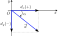
\includegraphics[width=0.75\textwidth]{figs/fig-05.png}
\end{center}
\begin{itemize}
    \item Las leyes de Newton sólo son válidas en marcos de referencia inerciales.
    \item Si un marco es inercial, otro que se mueve a velocidad constante respecto del primero también es inercial.
\end{itemize}
\end{frame}

\begin{frame}{Leyes de Newton}
    \textbf{Ejemplos:} ¿En cuál de las siguientes situaciones la fuerza neta sobre el cuerpo es cero:
    \begin{enumerate}[i)]
        \item Un avión que vuela al norte con rapidez constante de \qty{120}{m/s} y altitud constante;
        \item Un automóvil que sube en línea recta por una colina con pendiente de \ang{3}, a una rapidez constante de \qty{90}{km/h};
        \item Un halcón que se mueve en círculos con rapidez constante de \qty{20}{km/h} a una altura constante de \qty{15}{m} sobre un campo abierto;
        \item Una caja con superficies lisas, sin fricción, que está en la parte de atrás de un camión cuando éste acelera hacia adelante en un camino plano a \qty{5}{m/s^2}?
    \end{enumerate}
\end{frame}

\begin{frame}{Leyes de Newton}
    \begin{center} 
        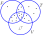
\includegraphics[scale=0.90]{figs/fig-06.pdf}

        La magnitud de la aceleración de un cuerpo es directamente proporcional a la magnitud de la fuerza neta que actúa sobre él.
    \end{center}
\end{frame}

\begin{frame}{Leyes de Newton}
\begin{columns}
\cx 
\begin{definition}[Masa]
    Llamamos \textbf{masa inercial} o simplemente \textbf{masa} al cociente de la magnitud de la fuerza neta que actúa sobre un cuerpo y la magnitud de la aceleración que le produce, y la denotamos con $m$:
    \[ m = \frac{\norm{\sum \vect{F}}}{\norm{\vect{a}}} \txt{o} \norm{\sum \vect{F}} = m a \txt{o} a = \frac{\norm{\sum \vect{F}}}{m} \]
\end{definition}
\cx 
\textbf{Unidades:}

\[ \qty{1}{N} = \qty{1}{kg} \cdot \unit{m/s^2} \]

\end{columns}
\pause

\begin{definition}[Segunda Ley de Newton]
    Si una fuerza externa actúa sobre un cuerpo, éste se acelera. La dirección de aceleración es la misma que la dirección de la fuerza neta. El vector de fuerza neta es igual a la masa del cuerpo multiplicada por su aceleración:
    \[ \sum \vect{F} = m \vect{a} \txt{en componentes:} \sum F_x = m a_x, \quad \sum F_y = m a_y, \quad  \sum F_z = m a_z \]
\end{definition}
\end{frame}

\begin{frame}{Leyes de Newton}
    \textbf{Ejemplo 1:} Un trabajador aplica una fuerza horizontal constante con magnitud de \qty{20}{N} a una caja con masa de \qty{40}{kg} que descansa en un piso plano con fricción despreciable. ¿Qué aceleración sufre la caja?

\begin{columns} 
\cw{0.4}
\begin{center} 
    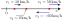
\includegraphics[width=1.0\textwidth]{figs/fig-07.png}
\end{center}
\pause 

\cw{0.6} 
\begin{align*}
    \sum F_x &= F = \qty{20}{N} = m a_x \\
    \sum F_y &= n - W = 0 = m a_y \Rightarrow a_y = 0
\end{align*}

\[ a_x = \frac{\sum F_x}{m} = \frac{\qty{20}{N}}{\qty{40}{kg}} = \frac{\qty{20}{kg \cdot m / s^2}}{\qty{40}{kg}} = \qty{0.50}{m/s^2} \]
\end{columns}

\end{frame}

\begin{frame}{Leyes de Newton}
    \textbf{Ejemplo 2:} Una persona empuja una botella de salsa de tomate con una masa de \qty{0.45}{kg} a la derecha sobre una mesa horizontal lisa. Al soltarla, la botella tiene una rapidez de \qty{2.8}{m/s}, pero se frena por la fuerza de fricción horizontal constante ejercida por la mesa. La botella se desliza \qty{1.0}{m} antes de detenerse. ¿Qué magnitud y dirección tiene la fuerza de fricción que actúa sobre la botella?

\begin{center} 
    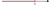
\includegraphics[width=0.7\textwidth]{figs/fig-08.png}
\end{center}
\pause 

\begin{columns}[t]
\cx 
\begin{align*}
    v_x^2 &= v_{0x}^2 + 2 a_x(x - x_0) \\
    a_x &= \frac{v_x^2 - v_{0x}^2}{2(x - x_0)} = \frac{(\qty{0}{m/s})^2 - (\qty{2.8}{m/s})^2}{2(\qty{1.0}{m} - 0\qty{0}{m})} = \qty{-3.9}{m/s^2} \\
\end{align*}
\cx 
\begin{align*}
    \sum F_x &= -f = m a_x = (\qty{0.45}{kg}) (\qty{-3.9}{m/s^2}) \\
             &= \qty{-1.8}{kg \cdot m/s^2} = \qty{-1.8}{N}
\end{align*}
\end{columns}
\end{frame}

\begin{frame}{Leyes de Newton}
\begin{columns}
\cw{0.6}
    \textbf{Masa y peso:}
    \begin{itemize}
        \item \textbf{Masa}: es la \textbf{inercia} de un cuerpo (tendencia a conservar su velocidad cuando se aplica una fuerza). Es una magnitud \textbf{escalar} que se mide en \unit{kg}. No depende del planeta en que se encuentre.
        \item \textbf{Peso}: es la \textbf{fuerza} de atracción que el planeta ejerce sobre un cuerpo. Es una magnitud \textbf{vectorial} y se mide en \unit{N}. Depende del planeta en que se encuentre el cuerpo.
        \item La masa se mide comparando, usando balanza de platillos.
        \item La fuerza se mide con balanza de resorte (dinamómetro).
        \item La aceleración se mide con metro y cronómetro.
        \item Cerca de la superficie terrestre, $g = \qty{9.8}{m/s^2}$ y apunta hacia el centro del planeta.
    \end{itemize}
    \[ \boxed{ \vect{P} = m \, \vect{g} } \]
\cw{0.4}
\begin{center}
    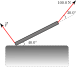
\includegraphics[scale=0.34]{figs/fig-09}\\
    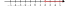
\includegraphics[scale=0.35]{figs/fig-10}
\end{center}
\end{columns}
\end{frame}

\begin{frame}{Leyes de Newton}
\begin{columns}
\cx 
\begin{definition}[Tercera Ley de Newton]
    Si un cuerpo $A$ ejerce una fuerza sobre un cuerpo $B$ (una \textbf{acción}), entonces el cuerpo $B$ ejerce una fuerza sobre $A$ (una \textbf{reacción}). Estas dos fuerzas tienen la misma magnitud y dirección, pero sentidos opuestos, y actúan sobre \alert{cuerpos diferentes}.

    \[ \boxed{\vect{F}_{A \text{ sobre } B} = - \vect{F}_{B \text{ sobre } A}} \]
\end{definition}

\cx 
\begin{center}
    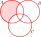
\includegraphics[width=0.8\textwidth]{figs/fig-11.png}
\end{center}

\begin{alertblock}{\centering \faExclamationTriangle}
    El par de fuerzas de acción y reacción actúan \alert{sobre cuerpos diferentes}. En problemas que implican la primera o segunda ley de Newton, no se deben sumar estos pares porque no actúan sobre el mismo cuerpo.
\end{alertblock}
\end{columns}
\end{frame}

\begin{frame}{Leyes de Newton}
    \textbf{Ejemplo:} una manzana esta en equilibrio sobre una mesa. ¿Qué fuerzas actúan sobre ella? ¿Cuál es la fuerza de reacción para cada una de ellas? ¿Cuáles son los pares acción-reacción?

    \begin{center}
        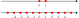
\includegraphics[scale=0.5]{figs/fig-12.png}
    \end{center}
\end{frame}




\end{document}
